\chapter{Mutações e diversificação dos genomas}\label{ch:b2:genome-diversification}

Espalhe um bilhão de bactérias numa placa impregnada de antibiótico e,
na manhã seguinte, um punhado de colônias terá crescido. O fármaco
ensinou essas células a resistir a ele, ou elas já eram resistentes
antes de encontrá-lo? A pergunta parece filosófica e foi resolvida em
1943 por um experimento de grande elegância: as células resistentes
já estavam lá antes, produzidas por \omterm{def:b2:genome-diversification:mutation}{mutações} que ocorreram ao acaso,
sem nenhuma relação com sua utilidade. Este capítulo trata das fontes
dessa variação --- os erros de cópia, os acidentes químicos, os genes
saltadores, os genes trocados entre células, as duplicações de genes
e de genomas inteiros --- e da velocidade com que operam. A seleção,
que tria a variação, é o assunto do
\cref{ch:b2:population-genetics}; aqui o assunto é de onde vem a matéria-prima.

\section{As mutações}

\begin{definition}[A mutação e seus tipos]\label{def:b2:genome-diversification:mutation}
\index{mutação}\index{mutação pontual}\index{deslocamento do quadro de leitura}\index{rearranjo cromossômico}
Uma \emph{mutação} é uma mudança hereditária na sequência do genoma.
As \emph{mutações pontuais} alteram uma ou poucas bases: uma
\emph{substituição} troca uma base por outra (uma \emph{transição}
troca purina por purina ou pirimidina por pirimidina,
A$\leftrightarrow$G ou C$\leftrightarrow$T; uma
\emph{transversão} troca as classes); uma \emph{inserção} ou uma
\emph{deleção} acrescenta ou remove bases. Numa sequência codificante,
uma substituição é \emph{silenciosa} se o novo códon especifica o
mesmo aminoácido, \emph{de sentido trocado} se especifica outro,
\emph{sem sentido} se cria um códon de parada; uma inserção ou deleção
que não seja múltipla de três desloca o quadro de leitura
(\emph{deslocamento do quadro de leitura}) e embaralha todos os códons
a jusante. Os \emph{rearranjos cromossômicos} deslocam grandes
segmentos: deleção, duplicação, inversão, translocação entre
cromossomos. As \emph{mutações genômicas} alteram o número de
cromossomos: \emph{aneuploidia} (um cromossomo a mais ou a menos, como
na trissomia do 21) e \emph{\omterm{def:b2:genome-diversification:polyploidy}{poliploidia}} (conjuntos inteiros a mais).
Uma mutação numa célula somática é herdada apenas pelos descendentes
dessa célula; uma mutação na linhagem germinativa é herdada pelos
descendentes do organismo, e só estas contam para a evolução.
\end{definition}

\begin{omfigure}
\begin{tikzpicture}[every node/.style={font=\small\ttfamily}]
  \node[anchor=west] at (0,2.4) {ATG GAA TTC CTG AAG TGG TAA};
  \node[anchor=west, font=\scriptsize\rmfamily] at (5.6,2.4) {Met Glu Phe Leu Lys Trp parada --- tipo selvagem};
  \node[anchor=west] at (0,1.7) {ATG GA\textcolor{omThm}{G} TTC CTG AAG TGG TAA};
  \node[anchor=west, font=\scriptsize\rmfamily] at (5.6,1.7) {Met Glu Phe Leu Lys Trp parada --- silenciosa};
  \node[anchor=west] at (0,1.0) {ATG G\textcolor{omThm}{T}A TTC CTG AAG TGG TAA};
  \node[anchor=west, font=\scriptsize\rmfamily] at (5.6,1.0) {Met \textcolor{omThm}{Val} Phe Leu Lys Trp parada --- sentido trocado};
  \node[anchor=west] at (0,0.3) {ATG \textcolor{omThm}{T}AA TTC CTG AAG TGG TAA};
  \node[anchor=west, font=\scriptsize\rmfamily] at (5.6,0.3) {Met \textcolor{omThm}{parada} --- sem sentido};
  \node[anchor=west] at (0,-0.4) {ATG GA\textcolor{omThm}{C}A TTC CTG AAG TGG TAA};
  \node[anchor=west, font=\scriptsize\rmfamily] at (5.6,-0.4) {Met \textcolor{omThm}{Asp Ile Pro Glu Val} \dots{} --- deslocamento do quadro};
\end{tikzpicture}

{\small \omterm{def:b2:genome-diversification:mutation}{Mutações pontuais} numa sequência codificante curta (a mudança
em vermelho). Uma substituição silenciosa conserva a proteína; uma de
sentido trocado muda um resíduo; uma sem sentido a trunca; uma única
base inserida desloca o quadro de leitura e reescreve tudo a jusante.}
\end{omfigure}

\begin{proposition}[De onde vêm as mutações]\label{prop:b2:genome-diversification:sources}
\index{mutágeno}\index{desaminação}\index{depurinação}
Há três fontes. \emph{Erros de replicação}: a DNA-polimerase coloca
uma base errada cerca de uma vez em $10^{5}$; sua exonuclease de
revisão remove a maioria, deixando uma em $10^{7}$; o reparo de
pareamento incorreto, que segue a forquilha de replicação e corrige a
fita nova com base na antiga, leva a taxa final de erro a cerca de
$10^{-9}$ a $10^{-10}$ por base por replicação. \emph{Química
espontânea}: todos os dias, em cada célula humana, cerca de
\num{10000} purinas se soltam de seus açúcares
(\emph{depurinação}) e uma centena de citosinas perde um grupo amino
(\emph{desaminação}, que transforma C em U, que pareia com A); ambas
são reparadas, mas nem sempre. \emph{Mutágenos}: a luz ultravioleta
solda timinas adjacentes em dímeros; a radiação ionizante quebra as
fitas; os agentes alquilantes e o ácido nitroso alteram bases; os
corantes intercalantes se insinuam entre os pares de bases e causam
\omterm{def:b2:genome-diversification:mutation}{deslocamentos do quadro de leitura}; os radicais de oxigênio da
respiração oxidam a guanina. A taxa por base é minúscula; multiplicada
pelo tamanho de um genoma e pelo número de células, deixa de ser.
\end{proposition}

\begin{theorem}[Mutações por genoma e por população]\label{thm:b2:genome-diversification:rate}
\index{taxa de mutação}
Se a \omterm{thm:b2:genome-diversification:rate}{taxa de mutação} é $u$ por par de bases por replicação e o genoma
contém $G$ pares de bases, cada replicação produz em média
$U = uG$ \omterm{def:b2:genome-diversification:mutation}{mutações} novas, e uma população de $N$ células produz $UN$
por geração. Para \emph{E.~coli} ($u \approx \qty{5e-10}{}$, $G =
\qty{4.6e6}{}$): $U \approx 0.002$, de modo que uma célula em cada
quinhentas carrega uma \omterm{def:b2:genome-diversification:mutation}{mutação} nova --- mas uma cultura de $10^{9}$
células produz dois milhões por geração, e cada uma das $3G \approx 1.4\times
10^{7}$ substituições de base única possíveis surge em algum lugar
dela a cada poucas gerações. Para um ser humano
($u \approx \qty{1.2e-8}{}$ por
geração, $G = \qty{3.2e9}{}$ por conjunto haploide, dois conjuntos):
cada criança carrega cerca de \num{75} \omterm{def:b2:genome-diversification:mutation}{mutações} novas, uma ou duas
delas em sequência codificante.
\end{theorem}
\begin{proof}
Cada base é copiada de modo independente, com probabilidade $u$ de
erro, de modo que o número de erros por cópia do genoma é uma soma de
$G$ eventos raros independentes, de média $uG$ (e com distribuição
aproximadamente de Poisson). $N$ células fazem $N$ cópias. O valor
humano multiplica $u$ por $2G$ para o genoma diploide; a taxa por
geração é por geração, e não por replicação, porque as células
germinativas passam por muitas replicações entre uma fecundação e a
seguinte.
\end{proof}

\begin{theorem}[Mutantes numa cultura em crescimento]\label{thm:b2:genome-diversification:luria}
\index{experimento de Luria--Delbrück}\index{teste de flutuação}
Uma cultura que cresce de $N_0$ a $N$ células, na qual uma dada
\omterm{def:b2:genome-diversification:mutation}{mutação} ocorre com probabilidade $m$ a cada divisão celular, contém
no final um número médio de \emph{eventos} de \omterm{def:b2:genome-diversification:mutation}{mutação} $m(N - N_0)$ e
um número médio de \emph{células} mutantes
\[
\langle M\rangle = m\,N\,\ln\frac{N}{N_0},
\]
maior que o número de eventos porque uma \omterm{def:b2:genome-diversification:mutation}{mutação} precoce funda um
clone. O número de células mutantes varia enormemente de uma cultura
para outra (os raros eventos precoces dão ``prêmios acumulados''), ao
passo que, se as \omterm{def:b2:genome-diversification:mutation}{mutações} fossem induzidas no plaqueamento, ele
seguiria uma lei de Poisson com variância igual à média. A fração de
culturas sem nenhum mutante é $p_0 = e^{-m(N - N_0)}$, o que dá $m$
diretamente.
\end{theorem}
\begin{proof}
O crescimento de $n$ para $n + \mathrm{d}n$ células exige
$\mathrm{d}n$ divisões, cada uma uma oportunidade para a \omterm{def:b2:genome-diversification:mutation}{mutação}, de
modo que ocorrem $m\,\mathrm{d}n$ eventos nesse intervalo; somando,
$m(N - N_0)$ eventos ao todo. Uma \omterm{def:b2:genome-diversification:mutation}{mutação} que ocorre quando a cultura
tem $n$ células funda um clone que cresce em sincronia com a cultura e
conta $N/n$ células no final; o número esperado de células mutantes é,
portanto,
$\int_{N_0}^{N} m\,(N/n)\,\mathrm{d}n = mN\ln(N/N_0)$. Os eventos são
raros e independentes, de modo que seu número segue uma lei de Poisson
de média $m(N - N_0)$, e a probabilidade de nenhum é
$e^{-m(N - N_0)}$.
\end{proof}
\begin{proof}[Evidências]
Luria e Delbrück (1943) cultivaram vinte pequenas culturas de
\emph{E.~coli}, cada uma a partir de poucas células, e em paralelo
retiraram vinte amostras de uma única cultura grande; plaquearam as
quarenta com um bacteriófago que mata toda célula sensível e contaram
as colônias resistentes. As amostras da cultura única deram contagens
próximas da média, como prevê uma lei de Poisson; as culturas
independentes deram contagens de 0, 0, 1, 0, 3, 0, 107, 0, 5\dots{}
--- uma variância muitas vezes maior que a média. As \omterm{def:b2:genome-diversification:mutation}{mutações} para a
resistência tinham ocorrido em momentos aleatórios \emph{antes} de as
células encontrarem o fago, e as precoces produziram os prêmios
acumulados. Lederberg e Lederberg (1952) confirmaram o resultado sem
nunca expor as células selecionadas ao agente: pressionando um
tampão de veludo sobre uma placa e carimbando cópias, encontraram
colônias resistentes nas mesmas posições em todas as réplicas, e as
isolaram da placa-mestra não tratada.
\end{proof}

\begin{omfigure}
\begin{tikzpicture}[every node/.style={font=\scriptsize}, level distance=0.55cm, sibling distance=0.5cm, edge from parent/.style={draw, gray}]
  \begin{scope}
    \node[circle, fill=omDef!40, inner sep=1.5pt] (r) at (0,0) {}
      child { node[circle, fill=omDef!40, inner sep=1.5pt] {}
        child { node[circle, fill=omDef!40, inner sep=1.5pt] {} child { node[circle, fill=omDef!40, inner sep=1.5pt] {} } child { node[circle, fill=omDef!40, inner sep=1.5pt] {} } }
        child { node[circle, fill=omDef!40, inner sep=1.5pt] {} child { node[circle, fill=omDef!40, inner sep=1.5pt] {} } child { node[circle, fill=omThm, inner sep=1.5pt] {} } } }
      child { node[circle, fill=omDef!40, inner sep=1.5pt] {}
        child { node[circle, fill=omDef!40, inner sep=1.5pt] {} child { node[circle, fill=omDef!40, inner sep=1.5pt] {} } child { node[circle, fill=omDef!40, inner sep=1.5pt] {} } }
        child { node[circle, fill=omDef!40, inner sep=1.5pt] {} child { node[circle, fill=omDef!40, inner sep=1.5pt] {} } child { node[circle, fill=omDef!40, inner sep=1.5pt] {} } } };
    \node[align=center] at (0,-2.4) {mutação tardia:\\uma célula mutante};
  \end{scope}
  \begin{scope}[xshift=5cm]
    \node[circle, fill=omDef!40, inner sep=1.5pt] at (0,0) {}
      child { node[circle, fill=omThm, inner sep=1.5pt] {}
        child { node[circle, fill=omThm, inner sep=1.5pt] {} child { node[circle, fill=omThm, inner sep=1.5pt] {} } child { node[circle, fill=omThm, inner sep=1.5pt] {} } }
        child { node[circle, fill=omThm, inner sep=1.5pt] {} child { node[circle, fill=omThm, inner sep=1.5pt] {} } child { node[circle, fill=omThm, inner sep=1.5pt] {} } } }
      child { node[circle, fill=omDef!40, inner sep=1.5pt] {}
        child { node[circle, fill=omDef!40, inner sep=1.5pt] {} child { node[circle, fill=omDef!40, inner sep=1.5pt] {} } child { node[circle, fill=omDef!40, inner sep=1.5pt] {} } }
        child { node[circle, fill=omDef!40, inner sep=1.5pt] {} child { node[circle, fill=omDef!40, inner sep=1.5pt] {} } child { node[circle, fill=omDef!40, inner sep=1.5pt] {} } } };
    \node[align=center] at (0,-2.4) {mutação precoce:\\um prêmio de quatro};
  \end{scope}
  \begin{scope}[xshift=10cm]
    \node[circle, fill=omDef!40, inner sep=1.5pt] at (0,0) {}
      child { node[circle, fill=omDef!40, inner sep=1.5pt] {}
        child { node[circle, fill=omDef!40, inner sep=1.5pt] {} child { node[circle, fill=omDef!40, inner sep=1.5pt] {} } child { node[circle, fill=omThm, inner sep=1.5pt] {} } }
        child { node[circle, fill=omDef!40, inner sep=1.5pt] {} child { node[circle, fill=omDef!40, inner sep=1.5pt] {} } child { node[circle, fill=omDef!40, inner sep=1.5pt] {} } } }
      child { node[circle, fill=omDef!40, inner sep=1.5pt] {}
        child { node[circle, fill=omDef!40, inner sep=1.5pt] {} child { node[circle, fill=omThm, inner sep=1.5pt] {} } child { node[circle, fill=omDef!40, inner sep=1.5pt] {} } }
        child { node[circle, fill=omDef!40, inner sep=1.5pt] {} child { node[circle, fill=omDef!40, inner sep=1.5pt] {} } child { node[circle, fill=omDef!40, inner sep=1.5pt] {} } } };
    \node[align=center] at (0,-2.4) {se induzidas no plaqueamento:\\dispersão de Poisson};
  \end{scope}
\end{tikzpicture}

{\small O \omterm{thm:b2:genome-diversification:luria}{teste de flutuação}. Se as \omterm{def:b2:genome-diversification:mutation}{mutações} (vermelho) ocorrem ao
acaso durante o crescimento, o número de mutantes depende de
\emph{quando} a \omterm{def:b2:genome-diversification:mutation}{mutação} aconteceu, e culturas independentes diferem
enormemente; se o agente seletivo as induzisse no plaqueamento, todas
as culturas mostrariam um número pequeno e parecido.}
\end{omfigure}

\begin{omfigure}
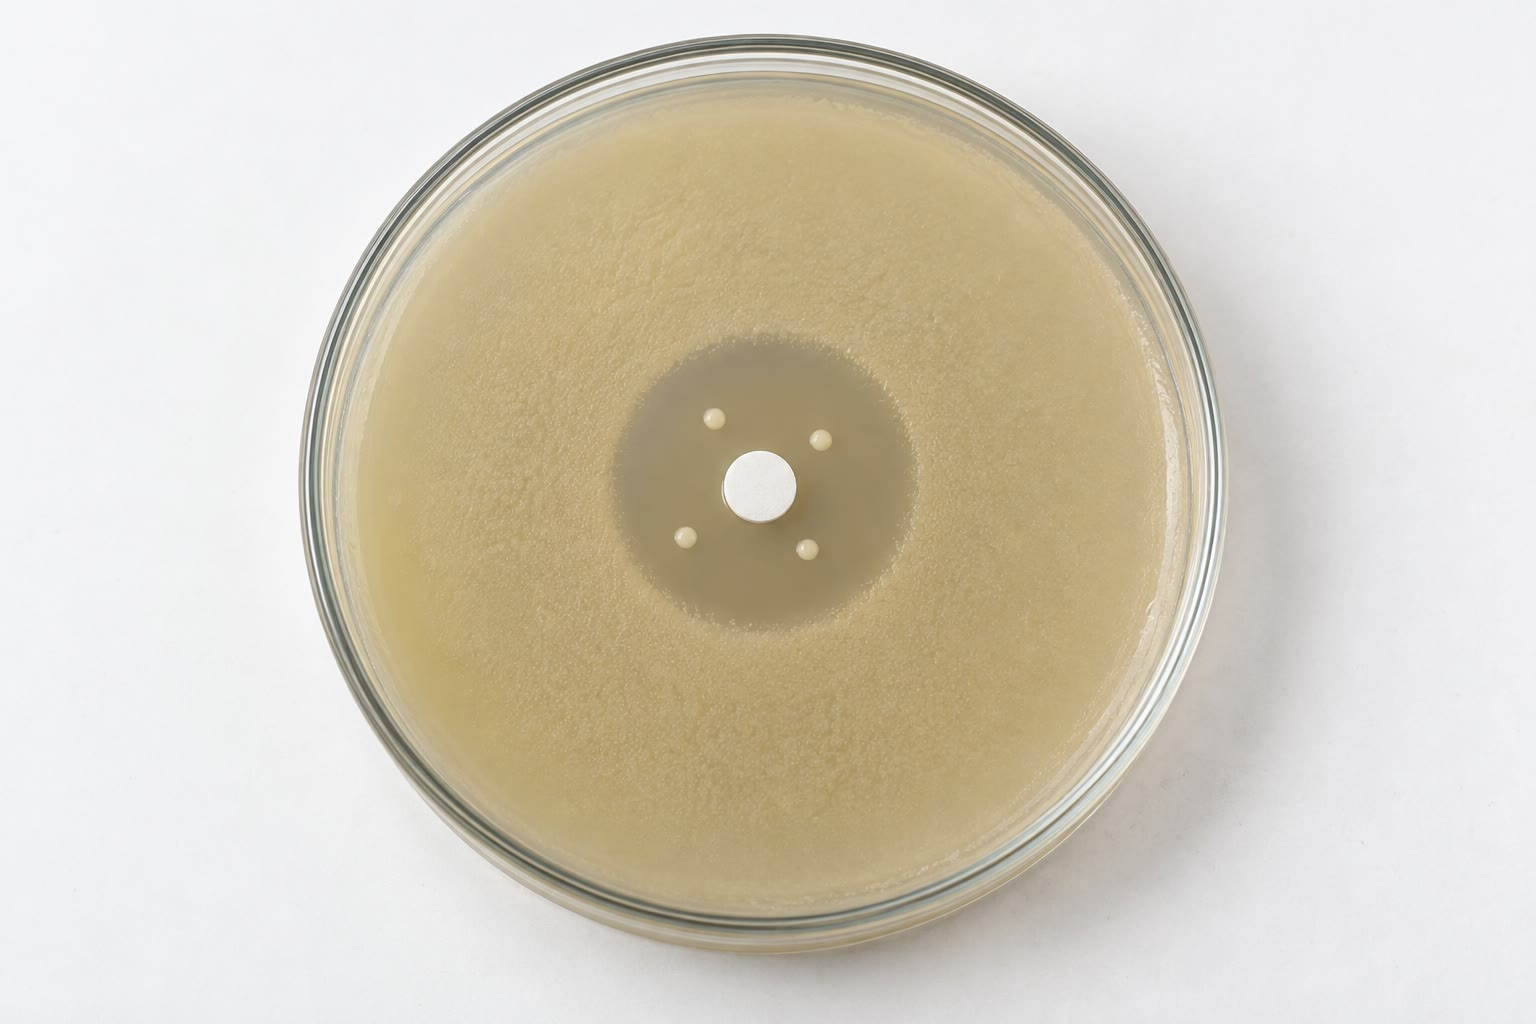
\includegraphics[width=0.5\linewidth]{images/book4/ai/b4-03-luria-plate.jpg}

{\small Um disco de antibiótico sobre um tapete de bactérias: a zona
clara é onde o fármaco que se difunde do disco matou as células
sensíveis, e as colônias dentro dela cresceram a partir de mutantes
resistentes que já estavam presentes antes de o disco ser colocado.}
\end{omfigure}

\begin{proposition}[O reparo e seus limites]\label{prop:b2:genome-diversification:repair}
\index{reparo do DNA}
Uma célula corrige a maior parte dos danos antes que se tornem
\omterm{def:b2:genome-diversification:mutation}{mutações}. O \emph{reparo de pareamento incorreto} remove a base errada
da fita recém-sintetizada. O \emph{reparo por excisão de bases} corta
uma única base danificada (uma uracila, uma guanina oxidada) e
preenche a lacuna; é por isso que o DNA usa timina e não uracila: uma
uracila no DNA só pode ser uma citosina desaminada, e é reconhecida
como estranha. O \emph{reparo por excisão de nucleotídeos} remove um
trecho de uma dúzia de bases em torno de uma lesão volumosa, como um
dímero de timina; as pessoas que não o têm (xeroderma pigmentoso)
desenvolvem cânceres de pele com a luz solar comum. O \emph{reparo por
recombinação} reconstrói um cromossomo quebrado a partir de sua cópia
irmã. O que escapa ao reparo, ou é reparado de forma errada, é uma
\omterm{def:b2:genome-diversification:mutation}{mutação} --- e uma célula que perdeu um sistema de reparo (uma
\emph{mutadora}) muta cem vezes mais depressa, o que é uma vantagem a
curto prazo sob estresse e um fardo a longo prazo. Os mecanismos de
reparo são tratados em profundidade no volume do Ano 3.
\end{proposition}

\section{Genes que se movem}

\begin{definition}[Elementos transponíveis]\label{def:b2:genome-diversification:transposon}
\index{transpóson}\index{retrotranspóson}
Um \emph{elemento transponível} é um segmento de DNA capaz de se mover
para uma nova posição no genoma. Os \emph{transpósons de DNA}
codificam uma \emph{transposase} que recorta o elemento e o cola em
outro lugar (ou o copia ali); as sequências de inserção bacterianas
são as mais simples (um gene de transposase entre duas repetições
invertidas), e os transpósons compostos carregam genes adicionais ---
muitas vezes de resistência a antibióticos --- entre duas delas. Os
\emph{retrotranspósons} se movem por uma via de copiar e colar através
de um intermediário de RNA, copiado de volta em DNA por uma
transcriptase reversa; nunca deixam o sítio antigo e, por isso, se
acumulam. Um elemento que cai dentro de um gene o interrompe; caindo
perto de um, pode alterar sua expressão; duas cópias num mesmo
cromossomo oferecem sítios para um \omterm{prop:b2:genome-diversification:duplication}{crossing-over desigual}. Os
transpósons e suas relíquias constituem metade do genoma humano e
oitenta por cento do genoma do milho; a maioria está hoje imóvel.
\end{definition}
\begin{proof}[Evidências]
McClintock (décadas de 1940 e 1950) estudou grãos de milho cujo
pigmento púrpura se perdia em algumas células e se restabelecia em
outras, produzindo grãos pintados. Mostrou, por cruzamentos e pela
observação dos cromossomos, que a instabilidade era causada por um
elemento (\emph{Dissociation}) que quebrava o cromossomo onde estava
e se movia entre posições sob o controle de um segundo elemento
(\emph{Activator}), e que um gene era silenciado quando o elemento
estava nele e reativado quando o elemento saía. Os genes, concluiu
ela, podiam mudar de posição; a ideia só foi aceita vinte anos depois,
quando se descobriram as sequências de inserção bacterianas, e lhe
valeu um Prêmio Nobel em 1983.
\end{proof}

\begin{omfigure}
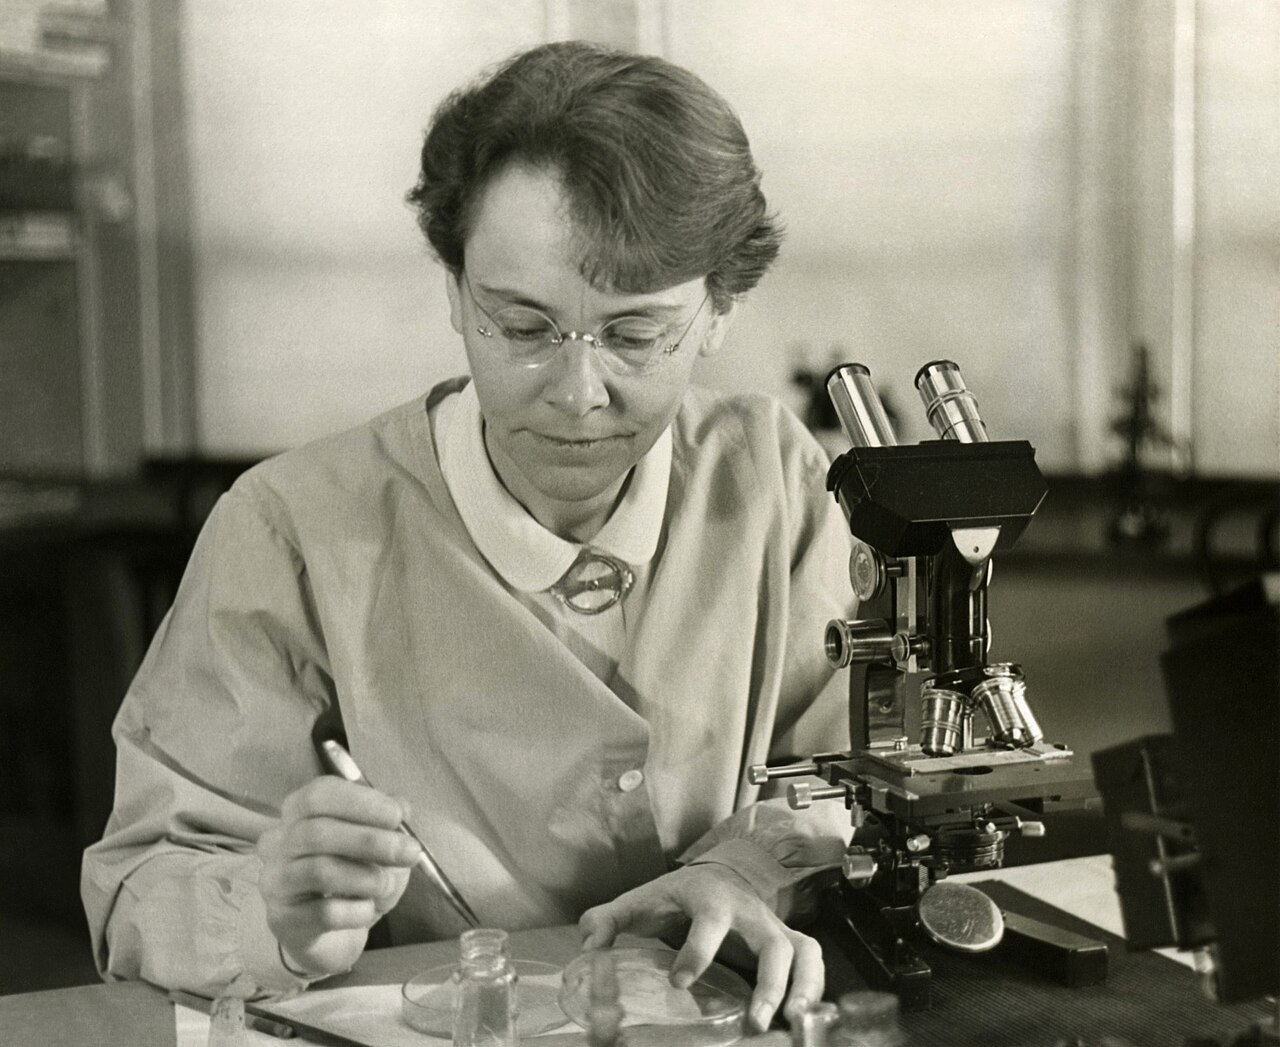
\includegraphics[width=0.4\linewidth]{images/book4/mcclintock.jpg}\hspace{0.04\linewidth}
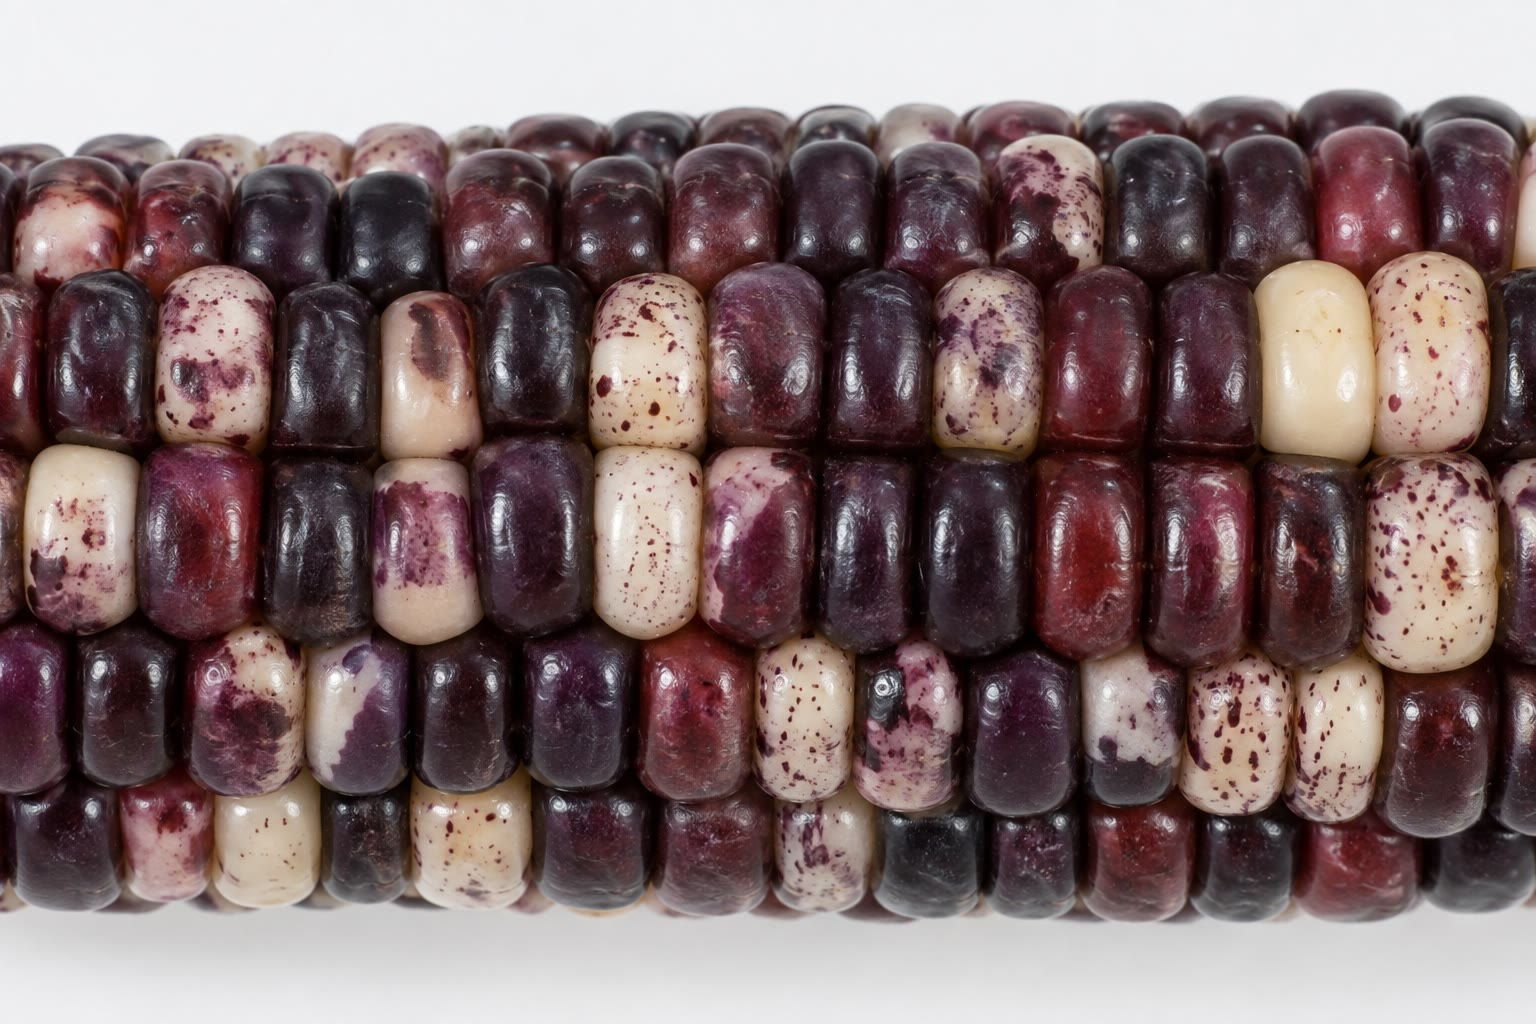
\includegraphics[width=0.5\linewidth]{images/book4/ai/b4-03-maize-kernels.jpg}

{\small Barbara McClintock e os grãos que a levaram aos elementos
transponíveis: um gene de pigmento púrpura desligado por um elemento
inserido e religado, célula por célula, quando o elemento salta para
fora, deixando pintas e setores.}
\end{omfigure}

\begin{omfigure}
\begin{tikzpicture}[every node/.style={font=\scriptsize}]
  % cut and paste
  \begin{scope}
    \draw[very thick, gray] (0,1.2) -- (4.5,1.2);
    \fill[omThm!70] (0.8,1.05) rectangle (1.8,1.35); \node[white, font=\tiny] at (1.3,1.2) {Tn};
    \draw[very thick, gray] (0,0) -- (4.5,0);
    \fill[omThm!70] (2.8,-0.15) rectangle (3.8,0.15); \node[white, font=\tiny] at (3.3,0) {Tn};
    \draw[->, thick, omThm] (1.3,1.0) .. controls (1.3,0.5) and (3.3,0.7) .. (3.3,0.2);
    \draw[dashed, gray] (0.8,1.2) -- (1.8,1.2);
    \node[align=center] at (2.25,-0.6) {recortar e colar (transpóson de DNA):\\o elemento deixa o sítio antigo};
  \end{scope}
  % copy and paste
  \begin{scope}[xshift=7.5cm]
    \draw[very thick, gray] (0,1.2) -- (4.5,1.2);
    \fill[omProp!80] (0.8,1.05) rectangle (1.8,1.35); \node[white, font=\tiny] at (1.3,1.2) {RT};
    \draw[very thick, gray] (0,0) -- (4.5,0);
    \fill[omProp!80] (2.8,-0.15) rectangle (3.8,0.15); \node[white, font=\tiny] at (3.3,0) {RT};
    \draw[->, thick, omProp] (1.3,1.0) .. controls (1.3,0.5) and (3.3,0.7) .. (3.3,0.2);
    \node[omProp, anchor=west, align=left] at (3.6,0.75) {cópia de RNA,\\retrotranscrita};
    \node[align=center] at (2.25,-0.6) {copiar e colar (retrotranspóson):\\a cópia antiga fica, o número cresce};
  \end{scope}
\end{tikzpicture}

{\small Duas maneiras de se mover. Um \omterm{def:b2:genome-diversification:transposon}{transpóson} de DNA é excisado e
reinserido; um \omterm{def:b2:genome-diversification:transposon}{retrotranspóson} é transcrito, copiado de volta em DNA e
inserido em outro lugar, de modo que suas cópias se acumulam.}
\end{omfigure}

\begin{definition}[Transferência horizontal de genes]\label{def:b2:genome-diversification:hgt}
\index{transferência horizontal de genes}\index{transformação}\index{conjugação!bacteriana}\index{transdução}
Os \omterm{def:b2:unicellular-diversity:prokaryote}{procariotos} adquirem genes de células que não são seus genitores
por três vias. \emph{Transformação}: uma célula capta DNA nu do meio
(liberado por células mortas) e o recombina em seu cromossomo; algumas
espécies são naturalmente competentes, e é por essa via que os
pneumococos trocam genes da cápsula. \emph{Conjugação}:
uma doadora portadora de um \omterm{def:b2:unicellular-diversity:prokaryote}{plasmídeo} conjugativo (o fator F de
\emph{E.~coli}) constrói um pilus, puxa uma receptora para perto e
passa uma única fita do \omterm{def:b2:unicellular-diversity:prokaryote}{plasmídeo} por um poro enquanto o replica pelo
mecanismo do círculo rolante; se o \omterm{def:b2:unicellular-diversity:prokaryote}{plasmídeo} se integrou ao cromossomo
(uma linhagem Hfr), genes cromossômicos são transferidos em ordem
atrás dele, e o momento em que cada um entra permite mapear o
cromossomo. \emph{Transdução}: um bacteriófago empacota por engano um
pedaço do DNA do hospedeiro e o injeta na próxima célula que infecta.
Juntas, essas vias transferem genes de resistência entre espécies
dentro dos hospitais em poucos anos, e transferiram genes metabólicos
por toda a árvore bacteriana ao longo do tempo geológico, de modo que
a ascendência de um \omterm{def:b2:unicellular-diversity:prokaryote}{procarioto} é tanto uma rede quanto uma árvore
(\cref{ch:b2:phylogenetic-trees}).
\end{definition}
\begin{proof}[Evidências]
Lederberg e Tatum (1946) misturaram duas linhagens de \emph{E.~coli},
cada uma incapaz de produzir dois nutrientes diferentes, e plaquearam
a mistura num meio mínimo em que nenhuma das duas podia crescer
sozinha: apareceram colônias, à razão de cerca de uma por dez milhões
de células, capazes de produzir os quatro --- recombinantes. Davis
(1950) repetiu o experimento com as linhagens separadas por um filtro
que deixava passar moléculas, mas não células: nenhum recombinante,
logo o contato era necessário. Hayes mostrou em seguida que a
transferência era unidirecional, de uma doadora para uma receptora, e
Wollman e Jacob (1956) interromperam os cruzamentos num liquidificador
a intervalos regulares e encontraram os genes da doadora entrando na
receptora numa ordem fixa, um após o outro, ao longo de cerca de cem
minutos.
\end{proof}

\begin{omfigure}
\begin{minipage}[b]{0.56\linewidth}\centering
\begin{tikzpicture}[every node/.style={font=\scriptsize}]
  % donor
  \draw[thick, fill=omDef!8] (0,0) ellipse (1.5 and 0.75);
  \draw[thick, omDef] (0.2,0) circle (0.45);
  \draw[thick, omThm] (-0.9,0.1) circle (0.22);
  \node[anchor=south] at (0,1.25) {doadora $F^+$};
  \draw[omThm] (-0.9,-0.12) -- (-1.1,-1.0) node[below] {plasmídeo F};
  \draw[omDef] (0.4,-0.4) -- (0.6,-1.0) node[below] {cromossomo};
  % recipient
  \draw[thick, fill=omDef!8] (5,0) ellipse (1.5 and 0.75);
  \draw[thick, omDef] (5.2,0) circle (0.45);
  \node[anchor=south] at (5,1.25) {receptora $F^-$};
  % pilus
  \draw[very thick, omThm] (1.5,0) -- (3.5,0);
  \node[omThm, below] at (2.5,-0.05) {pilus};
  % single strand transferred
  \draw[->, thick, omThm, dashed] (-0.7,0.15) .. controls (1.0,0.7) and (3.0,0.7) .. (4.1,0.4);
  \node[omThm, anchor=south] at (2.5,0.7) {uma fita copiada por círculo rolante};
  \draw[thick, omThm, dashed] (4.1,0.2) circle (0.2);
\end{tikzpicture}
\end{minipage}\hfill
\begin{minipage}[b]{0.42\linewidth}\centering
\begin{tikzpicture}
\begin{axis}[
  width=\linewidth, height=4.6cm,
  axis x line=bottom, axis y line=left,
  xmin=0, xmax=40, ymin=0, ymax=1.1,
  xlabel={minutos antes da agitação}, ylabel={recombinantes (relativo)},
  xlabel style={font=\scriptsize, at={(axis description cs:0.5,-0.18)}, anchor=north},
  ylabel style={font=\scriptsize},
  tick label style={font=\scriptsize}, xtick={0,10,20,30,40}, ytick={0,0.5,1},
  legend style={font=\scriptsize, at={(0.97,0.08)}, anchor=south east, draw=none},
  clip=false,
]
\addplot[very thick, omDef, domain=8:40, samples=40] {1-exp(-(x-8)/5)};
\addlegendentry{\emph{thr}, entra aos \qty{8}{min}}
\addplot[very thick, omProp, domain=17:40, samples=40] {1-exp(-(x-17)/5)};
\addlegendentry{\emph{lac}, \qty{17}{min}}
\addplot[very thick, omThm, domain=25:40, samples=40] {1-exp(-(x-25)/5)};
\addlegendentry{\emph{gal}, \qty{25}{min}}
\end{axis}
\end{tikzpicture}
\end{minipage}

{\small À esquerda: a conjugação --- a doadora passa uma fita de seu
\omterm{def:b2:unicellular-diversity:prokaryote}{plasmídeo} F através da junção do pilus enquanto a copia. À direita: o
experimento de cruzamento interrompido com uma doadora Hfr: cada gene
cromossômico começa a aparecer entre os recombinantes num momento
característico, o que mapeia o cromossomo em minutos.}
\end{omfigure}

\begin{omfigure}
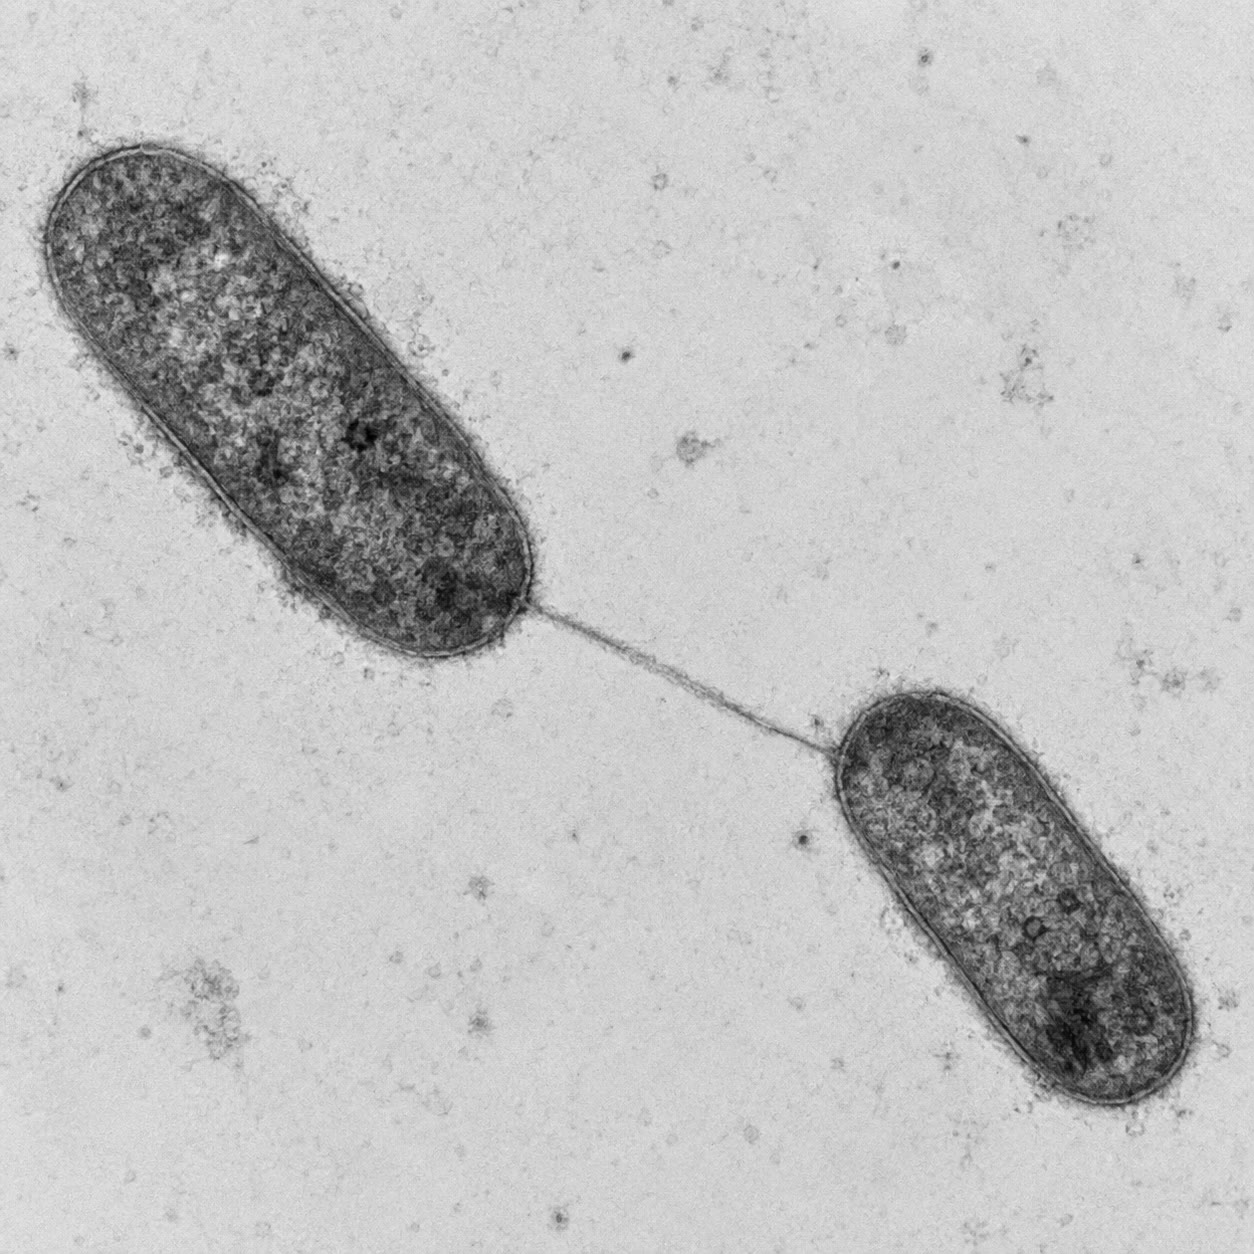
\includegraphics[width=0.42\linewidth]{images/book4/ai/b4-03-conjugation-tem.jpg}

{\small Duas bactérias unidas por um pilus conjugativo, vistas em
microscopia eletrônica de transmissão: a ponte ao longo da qual passa
o \omterm{def:b2:unicellular-diversity:prokaryote}{plasmídeo}.}
\end{omfigure}

\begin{example}[A resistência em movimento]\label{ex:b2:genome-diversification:resistance}
Um gene de resistência costuma surgir uma única vez, por \omterm{def:b2:genome-diversification:mutation}{mutação} ou a
partir da bactéria do solo que produz o antibiótico, e depois viaja:
de um cromossomo para um \omterm{def:b2:genome-diversification:transposon}{transpóson}, do \omterm{def:b2:genome-diversification:transposon}{transpóson} para um \omterm{def:b2:unicellular-diversity:prokaryote}{plasmídeo}
conjugativo, do \omterm{def:b2:unicellular-diversity:prokaryote}{plasmídeo} para outras espécies por conjugação e para
outras linhagens por \omterm{def:b2:genome-diversification:hgt}{transdução}, e de volta a um cromossomo por
\omterm{def:b2:genome-diversification:hgt}{transformação}. \omterm{def:b2:unicellular-diversity:prokaryote}{Plasmídeos} com cinco ou seis resistências ao mesmo
tempo (reunidas em \emph{integrons}, que capturam cassetes gênicos)
foram encontrados no Japão na década de 1950, poucos anos depois de os
fármacos entrarem em uso; o gene da carbapenemase NDM-1, visto pela
primeira vez em 2008, chegou a todos os continentes em três anos,
levado por um \omterm{def:b2:unicellular-diversity:prokaryote}{plasmídeo}. A evolução da resistência é, em grande parte,
não a evolução de genes novos, mas o deslocamento de genes antigos.
\end{example}

\section{Duplicação: genes e genomas}

\begin{proposition}[Duplicação gênica e famílias gênicas]\label{prop:b2:genome-diversification:duplication}
\index{duplicação gênica}\index{família gênica}\index{crossing-over desigual}
Quando duas sequências semelhantes estão em tandem num cromossomo, os
homólogos podem parear fora de registro na meiose e fazer um
\omterm{prop:b2:genome-diversification:duplication}{crossing-over desigual}, de modo que um produto carrega três cópias e o
outro, uma. Um gene duplicado é redundante: uma cópia pode manter a
função antiga enquanto a outra acumula \omterm{def:b2:genome-diversification:mutation}{mutações} livremente ---
geralmente degenerando num \emph{pseudogene}, ocasionalmente adquirindo
uma nova função (\emph{neofuncionalização}) ou uma parte da antiga
(\emph{subfuncionalização}). Repetido ao longo de centenas de milhões
de anos, esse processo constrói as \emph{\omterm{prop:b2:genome-diversification:duplication}{famílias gênicas}}: as
globinas (um único gene ancestral deu origem à mioglobina, ao
agrupamento $\alpha$ e ao agrupamento
$\beta$, com membros embrionários, fetais e adultos expressos
sucessivamente), os receptores olfativos (mil genes num camundongo),
os genes homeobox, as cristalinas do cristalino. A maioria dos genes
de um genoma pertence a uma família, e a duplicação é a principal
fonte de genes novos.
\end{proposition}
\begin{proof}[Evidências]
O agrupamento da $\beta$-globina humana, no cromossomo 11, contém cinco
genes funcionais ($\varepsilon$, $^{G}\gamma$, $^{A}\gamma$,
$\delta$, $\beta$) e um pseudogene, na ordem em que são ativados
durante o desenvolvimento, todos com a mesma estrutura de éxons e
íntrons, com sequências tanto mais parecidas quanto mais recente sua
divergência; o agrupamento $\alpha$, no cromossomo 16, tem a mesma
arquitetura. As deleções de um ou mais genes $\alpha$, produzidas por
\omterm{prop:b2:genome-diversification:duplication}{crossing-over desigual} entre as cópias quase idênticas, são comuns e
causam a $\alpha$-talassemia; o produto recíproco, um cromossomo com
três genes $\alpha$, é encontrado nas mesmas populações.
\end{proof}

\begin{omfigure}
\begin{tikzpicture}[every node/.style={font=\scriptsize}]
  % unequal crossing over
  \begin{scope}
    \draw[very thick, gray] (0,1.2) -- (5,1.2);
    \fill[omDef!70] (1.0,1.05) rectangle (2.0,1.35); \fill[omDef!70] (2.4,1.05) rectangle (3.4,1.35);
    \draw[very thick, gray] (0,0) -- (5,0);
    \fill[omDef!70] (1.0,-0.15) rectangle (2.0,0.15); \fill[omDef!70] (2.4,-0.15) rectangle (3.4,0.15);
    \node[above] at (1.5,1.35) {A}; \node[above] at (2.9,1.35) {A$'$};
    \draw[very thick, omThm] (2.9,1.05) -- (1.5,0.15);
    \node[align=center] at (2.5,-0.6) {homólogos mal pareados\\fazem crossing-over desigual};
    \draw[->, thick, gray] (5.3,0.6) -- (6.1,0.6);
    % products
    \draw[very thick, gray] (6.5,1.2) -- (11.5,1.2);
    \fill[omDef!70] (7.5,1.05) rectangle (8.5,1.35); \fill[omDef!70] (8.9,1.05) rectangle (9.9,1.35); \fill[omDef!70] (10.3,1.05) rectangle (11.3,1.35);
    \node[above] at (9.4,1.35) {três cópias};
    \draw[very thick, gray] (6.5,0) -- (11.5,0);
    \fill[omDef!70] (7.5,-0.15) rectangle (8.5,0.15);
    \node[above] at (8.0,0.15) {uma cópia};
  \end{scope}
  % globin family tree
  \begin{scope}[yshift=-3.6cm]
    \draw[thick] (2,2.2) -- (2,1.7);
    \draw[thick] (0.5,1.7) -- (3.5,1.7);
    \draw[thick] (0.5,1.7) -- (0.5,0.4); \node[below] at (0.5,0.4) {mioglobina};
    \draw[thick] (3.5,1.7) -- (3.5,1.2);
    \draw[thick] (2.3,1.2) -- (4.7,1.2);
    \draw[thick] (2.3,1.2) -- (2.3,0.4); \node[below] at (2.3,0.4) {família $\alpha$};
    \draw[thick] (4.7,1.2) -- (4.7,0.9);
    \draw[thick] (3.6,0.9) -- (5.8,0.9);
    \draw[thick] (3.6,0.9) -- (3.6,0.4); \node[below] at (3.6,0.4) {$\varepsilon,\gamma$};
    \draw[thick] (5.8,0.9) -- (5.8,0.7);
    \draw[thick] (5.2,0.7) -- (6.4,0.7);
    \draw[thick] (5.2,0.7) -- (5.2,0.4); \node[below] at (5.2,0.4) {$\delta$};
    \draw[thick] (6.4,0.7) -- (6.4,0.4); \node[below] at (6.4,0.4) {$\beta$};
    \node[anchor=west, align=left] at (7.2,1.7) {duplicações de um gene ancestral de globina:\\antes dos vertebrados (mioglobina/hemoglobina),\\há $\sim$450 milhões de anos ($\alpha$/$\beta$),\\depois dentro do agrupamento $\beta$ (embrionária, fetal, adulta)};
    \node[anchor=east, gray] at (1.9,2.1) {globina ancestral};
  \end{scope}
\end{tikzpicture}

{\small Acima: o \omterm{prop:b2:genome-diversification:duplication}{crossing-over desigual} entre cópias em tandem mal
pareadas produz um cromossomo com três cópias e outro com uma só.
Abaixo: a família das globinas, construída por duplicações e
divergências sucessivas.}
\end{omfigure}

\begin{definition}[Poliploidia]\label{def:b2:genome-diversification:polyploidy}
\index{poliploidia}\index{alopoliploide}\index{autopoliploide}
Um \emph{poliploide} tem mais de dois conjuntos cromossômicos
completos. Um \emph{autopoliploide} tem vários conjuntos de uma mesma
espécie (uma meiose falha dá um gameta diploide; dois desses gametas
dão um tetraploide); um \emph{alopoliploide} reúne os conjuntos de duas
espécies após uma hibridização. O híbrido diploide AB, sem homólogo
para nenhum cromossomo, não consegue pareá-los na meiose e é estéril;
se seu genoma se duplica em AABB, cada cromossomo volta a ter um par,
a meiose funciona e a nova planta é fértil --- mas não consegue se
cruzar de volta com nenhum dos genitores (um descendente AAB é
estéril). A poliploidia faz, assim, uma nova espécie num único passo,
e cerca de um terço das espécies de plantas com flores surgiu dessa
maneira: o trigo-mole é um hexaploide AABBDD de três gramíneas, o
morango cultivado um octoploide, o algodão e o tabaco alotetraploides,
e a própria linhagem dos vertebrados duplicou seu genoma duas vezes
perto de sua origem. Os poliploides costumam ser maiores que seus
ancestrais diploides (mais DNA, células maiores) e são muito
apreciados pelos melhoristas.
\end{definition}

\begin{omfigure}
\begin{tikzpicture}[every node/.style={font=\scriptsize}]
  \node[draw, rounded corners, fill=omDef!10, align=center] (a) at (0,0) {\emph{T.~urartu}\\AA, $2n = 14$};
  \node[draw, rounded corners, fill=omDef!10, align=center] (b) at (3.4,0) {\emph{Aegilops}\\BB, $2n = 14$};
  \node[draw, rounded corners, fill=omProp!15, align=center] (ab) at (1.7,-1.5) {híbrido AB\\$n = 14$, estéril};
  \node[draw, rounded corners, fill=omExo!25, align=center] (aabb) at (1.7,-3.1) {trigo emmer AABB\\$2n = 28$, fértil};
  \node[draw, rounded corners, fill=omDef!10, align=center] (d) at (6.4,-3.1) {\emph{Ae.~tauschii}\\DD, $2n = 14$};
  \node[draw, rounded corners, fill=omProp!15, align=center] (abd) at (4.0,-4.6) {híbrido ABD\\$3n = 21$, estéril};
  \node[draw, rounded corners, fill=omExo!25, align=center] (abd2) at (4.0,-6.1) {trigo-mole AABBDD\\$2n = 42$, fértil};
  \draw[->, thick] (a) -- (ab); \draw[->, thick] (b) -- (ab);
  \draw[->, thick] (ab) -- (aabb) node[midway, right] {duplicação do genoma};
  \draw[->, thick] (aabb) -- (abd); \draw[->, thick] (d) -- (abd);
  \draw[->, thick] (abd) -- (abd2) node[midway, right] {duplicação do genoma};
  \node[anchor=west, align=left, gray] at (7.8,-1.5) {cada hibridização dá uma planta\\estéril com cromossomos sem par;\\cada duplicação restaura o\\pareamento e a fertilidade --- e faz\\uma espécie que não se cruza de volta};
\end{tikzpicture}

{\small A origem do trigo-mole: duas hibridizações, cada uma seguida
de uma duplicação do genoma, construíram um hexaploide a partir de três
gramíneas diploides em cerca de dez mil anos.}
\end{omfigure}

\begin{omfigure}
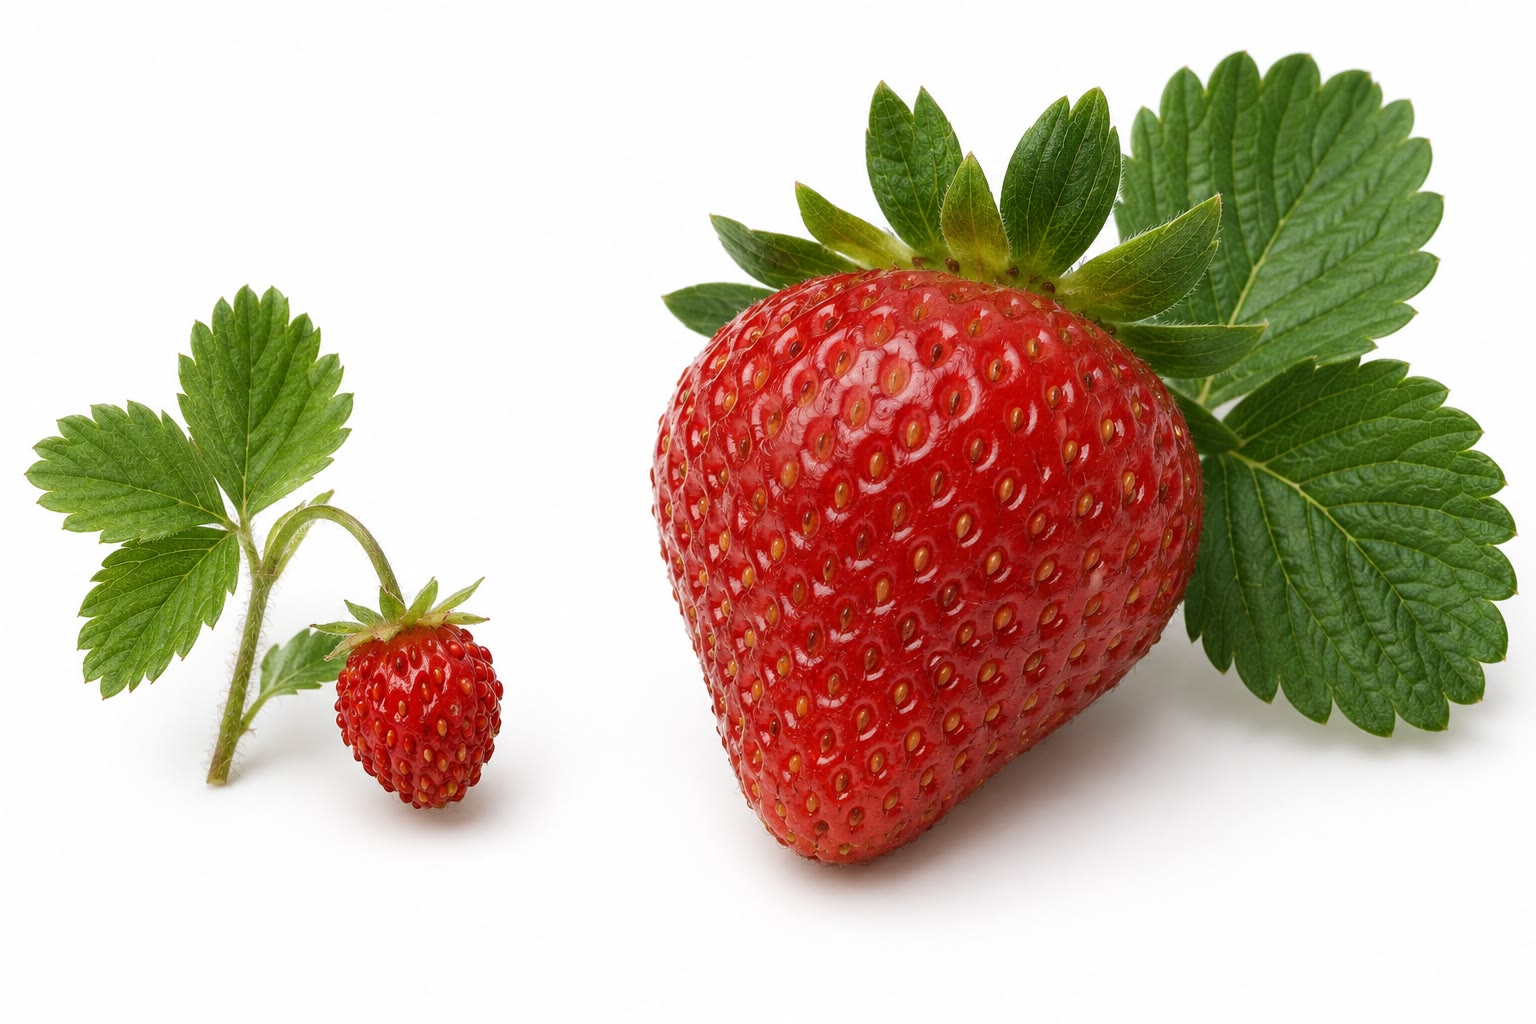
\includegraphics[width=0.55\linewidth]{images/book4/ai/b4-03-polyploid-strawberries.jpg}

{\small Um morango silvestre diploide e o octoploide cultivado: o
\omterm{def:b2:genome-diversification:polyploidy}{poliploide}, com quatro vezes mais DNA em cada célula, é a planta maior,
de fruto maior.}
\end{omfigure}

\section{Acaso e taxa}

\begin{proposition}[A mutação é aleatória em relação à necessidade]\label{prop:b2:genome-diversification:random}
\index{mutação!aleatoriedade da}
O \omterm{thm:b2:genome-diversification:luria}{teste de flutuação} e o plaqueamento em réplica mostram que uma
\omterm{def:b2:genome-diversification:mutation}{mutação} útil num ambiente novo surge com a mesma taxa, esteja o
ambiente presente ou não: o ambiente seleciona entre as \omterm{def:b2:genome-diversification:mutation}{mutações}, não
as provoca. A \omterm{def:b2:genome-diversification:mutation}{mutação} não é aleatória em todos os sentidos --- as
transições são mais numerosas que as transversões, os dinucleotídeos
CpG mutam dez vezes mais depressa que os outros sítios (sua citosina
metilada se desamina em timina, que o reparo não reconhece como
estranha), algumas regiões são pontos quentes, e o estresse pode
elevar a taxa global ---, mas é cega às consequências. A própria \omterm{thm:b2:genome-diversification:rate}{taxa
de mutação} é um caráter hereditário, e a seleção a ajusta: alta
demais, cada geração herda mudanças nocivas; baixa demais, a população
não consegue acompanhar um mundo em mudança. As linhagens mutadoras
vencem por pouco tempo num hospital e perdem a longo prazo, e a taxa de
$10^{-9}$ por base em que a maioria das células se estabiliza é um
compromisso entre o custo dos erros e o custo da revisão.
\end{proposition}

\section{Exercícios}

\begin{exercise}[$\star$]\label{exo:b2:genome-diversification:1}
Classifique cada mudança no códon GAA (glutamato): GAG; GTA; TAA;
inserção de um C após a primeira base. Qual é uma transição, e qual
uma transversão?
\end{exercise}

\begin{exercise}[$\star$]\label{exo:b2:genome-diversification:2}
Com $u = \qty{5e-10}{}$ por par de bases por replicação e $G =
\qty{4.6e6}{}$, quantas \omterm{def:b2:genome-diversification:mutation}{mutações} novas uma divisão de \emph{E.~coli}
produz em média? Quantas por geração numa cultura de
$10^{9}$ células?
\end{exercise}

\begin{exercise}[$\star$]\label{exo:b2:genome-diversification:3}
Cite as três vias de \omterm{def:b2:genome-diversification:hgt}{transferência horizontal de genes} e diga, para
cada uma, o que ela exige (contato, um vírus, DNA livre) e o que
costuma transferir.
\end{exercise}

\begin{exercise}[$\star$]\label{exo:b2:genome-diversification:4}
Distinga autopoliploidia de alopoliploidia, com um exemplo de cada, e
explique por que um híbrido diploide de duas espécies costuma ser
estéril.
\end{exercise}

\begin{exercise}[$\star\star$]\label{exo:b2:genome-diversification:5}
Uma linhagem germinativa humana acumula $u = \qty{1.2e-8}{}$ \omterm{def:b2:genome-diversification:mutation}{mutações}
por par de bases por geração num genoma haploide de \qty{3.2e9}{}
pares de bases. Quantas \omterm{def:b2:genome-diversification:mutation}{mutações} novas uma criança carrega? Se
\qty{1.5}{\%} do genoma codifica proteínas e \qty{70}{\%} das
substituições codificantes mudam um aminoácido, quantas mudanças novas
de aminoácido a criança carrega?
\end{exercise}

\begin{exercise}[$\star\star$]\label{exo:b2:genome-diversification:6}
Uma cultura cresce de $10^{3}$ a $10^{9}$ células; uma dada \omterm{def:b2:genome-diversification:mutation}{mutação}
ocorre a $m = \qty{2e-8}{}$ por divisão. Calcule o número esperado de
eventos de \omterm{def:b2:genome-diversification:mutation}{mutação} e de células mutantes. Por que a fração de culturas
sem mutante é inútil aqui para medir $m$, e que tamanho de cultura a
tornaria útil?
\end{exercise}

\begin{exercise}[$\star\star$]\label{exo:b2:genome-diversification:7}
A citosina se desamina em uracila; a 5-metilcitosina se desamina em
timina. Explique por que a primeira lesão é reparada com eficiência e
a segunda não, e deduza por que os sítios CpG (onde a citosina é
metilada) são pontos quentes de \omterm{def:b2:genome-diversification:mutation}{mutação} e são mais raros no genoma do
que o acaso preveria.
\end{exercise}

\begin{exercise}[$\star\star$]\label{exo:b2:genome-diversification:8}
Num experimento de cruzamento interrompido, quatro genes entram na
receptora aos 8, 17, 25 e \qty{40}{min}; o cromossomo inteiro
(\qty{4.6}{Mb}) levaria \qty{100}{min}. Converta os tempos em posições
em quilobases e calcule as distâncias entre genes consecutivos.
\end{exercise}

\begin{exercise}[$\star\star$]\label{exo:b2:genome-diversification:9}
Desenhe o pareamento e o crossing-over que transformam dois
cromossomos com dois genes de $\alpha$-globina em tandem cada um num
cromossomo com três e noutro com um. Uma pessoa herda um cromossomo
com um só gene de cada genitor: quantos genes $\alpha$ ela tem, e o
que se espera de sua hemoglobina?
\end{exercise}

\begin{exercise}[$\star\star\star$]\label{exo:b2:genome-diversification:10}
O trigo-mole é AABBDD, com $2n = 42$. Dê o número de cromossomos de
seus gametas, dos híbridos estéreis em cada etapa de sua origem e de
um cruzamento entre o trigo-mole e o trigo emmer (AABB). Explique, em
termos de pareamento meiótico, por que cada duplicação restaurou a
fertilidade e por que o hexaploide não consegue se cruzar de volta com
seus genitores.
\end{exercise}

\begin{exercise}[$\star\star\star$]\label{exo:b2:genome-diversification:11}
Numa população intestinal de $N = 10^{9}$ bactérias, um \omterm{def:b2:unicellular-diversity:prokaryote}{plasmídeo} de
resistência se espalha por conjugação a uma taxa proporcional aos
encontros entre portadoras $R$ e não portadoras $N - R$:
$\mathrm{d}R/\mathrm{d}t =
\gamma R (N - R)$ com $\gamma N = \qty{0.5}{h^{-1}}$. Resolva, partindo
de uma portadora, e calcule o tempo para que metade da população
carregue o \omterm{def:b2:unicellular-diversity:prokaryote}{plasmídeo}. O que acontece se o antibiótico for então
retirado e o \omterm{def:b2:unicellular-diversity:prokaryote}{plasmídeo} custar a sua hospedeira \qty{5}{\%} da taxa de
crescimento?
\end{exercise}

\begin{exercise}[$\star\star\star$]\label{exo:b2:genome-diversification:12}
``A \omterm{def:b2:genome-diversification:mutation}{mutação} é aleatória; a evolução não.'' Discuta, usando o \omterm{thm:b2:genome-diversification:luria}{teste de
flutuação}, o plaqueamento em réplica e o fato de que a própria \omterm{thm:b2:genome-diversification:rate}{taxa de
mutação} está sob seleção.
\end{exercise}

\section{Problema: Um teste de flutuação}

\begin{problem}[{Problema de fim de semana --- um teste de flutuação é
realizado e analisado, a taxa de mutação de uma linhagem é extraída
dele e levada à escala de seu genoma e de sua população, a
disseminação de um plasmídeo de resistência é modelada e o custo de
uma mutadora é avaliado, até a taxa de mutação por base da linhagem e
o tempo que o plasmídeo leva para dominar}]
\label{pb:b2:genome-diversification:1}
Vinte culturas de \emph{E.~coli} são iniciadas, cada uma, com \num{100}
células em \qty{0.2}{mL} e cultivadas até $N = \qty{2e8}{}$ células;
cada uma é então espalhada numa placa com um bacteriófago, e as
colônias resistentes são contadas: 0, 0, 0, 1, 0, 0, 3, 0, 0, 1, 0, 0,
0, 0, 107, 0, 2, 0, 0, 5. Em paralelo, vinte amostras de
\qty{0.2}{mL} são retiradas de uma única cultura grande, com a mesma
densidade, e plaqueadas da mesma forma:
14, 15, 13, 21, 15, 14, 26, 16, 20, 13, 17, 12, 18, 14, 16, 19, 15,
13, 17, 16. Genoma: \qty{4.6e6}{} pares de bases, \qty{88}{\%}
codificante. A resistência ao fago pode surgir por qualquer uma de
\num{20} substituições de base única distintas num gene de receptor.

\medskip
\noindent\textbf{Parte I --- O teste.}
\begin{enumerate}
  \item Calcule a média e a variância das vinte culturas
        independentes.
  \item Calcule a média e a variância das vinte amostras.
  \item Para uma distribuição de Poisson, a variância é igual à média.
        Qual conjunto segue Poisson, e o que a distribuição de cada
        conjunto diz sobre \emph{quando} as \omterm{def:b2:genome-diversification:mutation}{mutações} ocorreram?
  \item Explique a contagem de 107.
  \item Quantas das culturas independentes não contêm nenhum mutante?
        Use $p_0 = e^{-m(N - N_0)}$ para estimar $m$, a \omterm{thm:b2:genome-diversification:rate}{taxa de mutação}
        para a resistência por divisão celular.
  \item Calcule o número esperado de células mutantes por cultura a
        partir de $mN\ln(N/N_0)$ e compare com a média observada.
  \item Por que as amostras da cultura única teriam sido inúteis para
        estimar $m$ pelo método de $p_0$?
\end{enumerate}

\medskip
\noindent\textbf{Parte II --- Levando à escala do genoma.}
\begin{enumerate}[resume]
  \item Deduza a \omterm{thm:b2:genome-diversification:rate}{taxa de mutação} $u$ por par de bases por replicação a
        partir de $m$ e do número de mudanças que conferem resistência.
  \item Calcule o número médio de \omterm{def:b2:genome-diversification:mutation}{mutações} novas por genoma por
        replicação, $U$.
  \item Uma cultura de um litro a $10^{9}$ células por mililitro se
        duplica uma vez. Quantas \omterm{def:b2:genome-diversification:mutation}{mutações} novas surgem na população?
  \item Quantas substituições de base única distintas são possíveis
        nesse genoma? Em média, quantas vezes cada uma surge nessa única
        duplicação?
  \item Explique por que, numa população assim, a resistência a
        qualquer antibiótico isolado que uma única \omterm{def:b2:genome-diversification:mutation}{mutação} possa
        vencer está praticamente garantida.
  \item Explique por que combinar dois antibióticos que exigem duas
        \omterm{def:b2:genome-diversification:mutation}{mutações} independentes muda a situação, com um número.
\end{enumerate}

\medskip
\noindent\textbf{Parte III --- Um \omterm{def:b2:unicellular-diversity:prokaryote}{plasmídeo} se espalha.}
Num intestino com $N = 10^{9}$ células, uma célula adquire um
\omterm{def:b2:unicellular-diversity:prokaryote}{plasmídeo} de resistência conjugativo. As portadoras $R$ o transmitem
por contato:
$\mathrm{d}R/\mathrm{d}t = \gamma R(N - R)$, com $\gamma N =
\qty{0.5}{h^{-1}}$.
\begin{enumerate}[resume]
  \item Mostre que $R(t) = N/\bigl(1 + (N - 1)e^{-\gamma N t}\bigr)$
        é solução da equação com $R(0) = 1$.
  \item Calcule o instante em que metade das células carrega o
        \omterm{def:b2:unicellular-diversity:prokaryote}{plasmídeo}.
  \item Calcule o instante em que \qty{99}{\%} o carregam.
  \item Quantos eventos de conjugação por hora ocorrem no momento em
        que metade das células é portadora?
  \item Compare com o tempo para que um \emph{mutante} resistente
        alcance metade da população crescendo \qty{10}{\%} mais
        depressa que o restante sob o antibiótico (\omterm{def:b2:unicellular-diversity:division}{tempo de geração} de
        \qty{1}{h} para as células sensíveis): partindo de uma célula,
        quanto tempo isso leva?
  \item Conclua por que a resistência se espalha sobretudo por
        transferência, e não por descendência.
\end{enumerate}

\medskip
\noindent\textbf{Parte IV --- Uma mutadora.}
Uma linhagem sem reparo de pareamento incorreto muta \num{100} vezes
mais depressa. Suponha que \qty{30}{\%} das \omterm{def:b2:genome-diversification:mutation}{mutações} em sequência
codificante sejam nocivas.
\begin{enumerate}[resume]
  \item Calcule seu $U$ e o número médio de \omterm{def:b2:genome-diversification:mutation}{mutações} nocivas por
        célula por geração.
  \item Após \num{200} gerações, que fração dos descendentes de uma
        linhagem não carrega nenhuma \omterm{def:b2:genome-diversification:mutation}{mutação} nociva (Poisson)?
  \item Calcule o mesmo para o tipo selvagem.
  \item No \omterm{thm:b2:genome-diversification:luria}{teste de flutuação} acima, que contagem média a mutadora
        teria dado, e que fração de culturas sem mutante?
  \item Explique em duas frases por que as mutadoras são encontradas
        entre os isolados hospitalares e são raras na natureza.
  \item Enuncie o resultado: $m$, $u$, $U$ da linhagem, e os tempos
        para que o \omterm{def:b2:unicellular-diversity:prokaryote}{plasmídeo} alcance metade e \qty{99}{\%} do
        intestino.
\end{enumerate}
\end{problem}
